\documentclass[a4paper]{article}
\usepackage[14pt]{extsizes}
\usepackage[utf8]{inputenc}

\usepackage[russian]{babel}
\addto\captionsrussian{\renewcommand{\figurename}{Рисунок}}

\usepackage{caption}
\captionsetup{justification = raggedright,
	          singlelinecheck = false,
              font = {small, it}}

\usepackage[left=20mm, top=15mm, right=15mm, bottom=15mm, nohead, footskip=10mm]{geometry}

\usepackage{amsmath}
\usepackage{amsfonts}
\usepackage{booktabs}
\usepackage{siunitx}

\usepackage{graphicx}
\graphicspath{{./images/}}
\DeclareGraphicsExtensions{.png}

\usepackage{adjustbox, array}

\usepackage{dcolumn}
\newcolumntype{M}[1]{>{\centering\arraybackslash}m{#1}}

\usepackage{titlesec}
\titleformat{\section}{\normalfont\fontsize{17}{0}\selectfont\bfseries}{\thesection}{}{}
\titleformat{\subsection}{\normalfont\fontsize{14}{0}\selectfont\bfseries}{\thesection}{}{}

\usepackage{setspace}

\usepackage{enumitem}
\setlist{nolistsep, topsep=8pt, parsep=3pt, leftmargin=1.5cm}

\renewcommand{\labelitemi}{$ \circ $\hspace{0.225em}}

\begin{document}
	
	\begin{center}
		
		\  \vskip 10cm
		
		\fontsize{20}{18} \selectfont {Лабораторная работа № 6: Градуировка спектрометра}
		
		\vskip 0.5mm
		
		\fontsize{14}{16} \selectfont {
			
			\textit{Соболев Павел, 291 группа} \\
		    \textit{20.02.2019}
		    
		}
		
		\thispagestyle{empty}
		\newpage
		
	\end{center}

	\section*{Введение}
	
		\begin{flushleft}
		
			\fontsize{14}{0pt} \selectfont \textbf{\textit{Цели работы}}
			
			\begin{enumerate}
					
					\item Градуировка спектрометра
					\item Определение газа по спектру
	
			\end{enumerate}
		
			\fontsize{14}{0pt} \selectfont \textbf{\textit{Задачи работы}}
			
			\begin{enumerate}
				
				\item Проградуировать спектрометр по спектру ртути
				\item Получить градуировочную кривую
				\item Получить спектр газа
				\item Определить газ по спектру
				
			\end{enumerate}
		
			\fontsize{14}{0pt} \selectfont \textbf{\textit{Оборудование}}
			
			\begin{itemize}
				
				\item Монохроматор УМ-2
				\item Линза-конденсор
				\item Оптическая скамья
				\item Источник света (для юстировки)
				\item Ртутная лампа
				\item Лампа с газом
				
			\end{itemize}
		
		\end{flushleft}
	
		\newpage
		
	\section*{Оптические схемы}
	
		\begin{figure}[h]
			
			\vskip -0.5cm
			
			\caption{Оптическая схема монохроматора}
			
			\raisebox{-.5\height}{%
				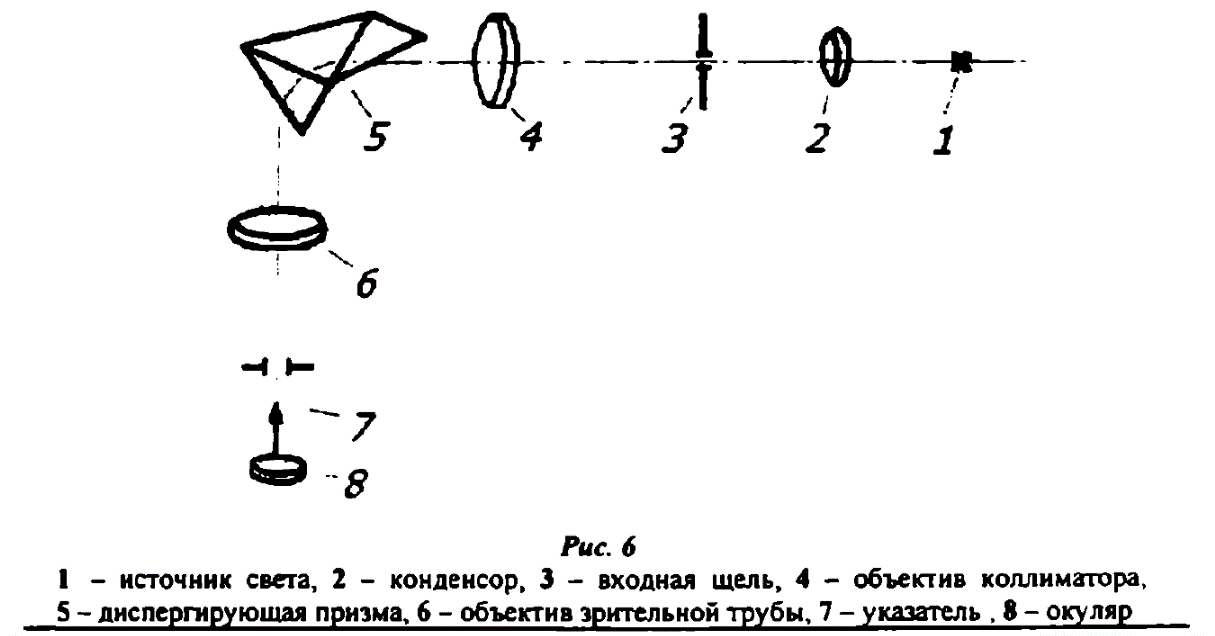
\includegraphics[scale=0.5]{1}%
			}
		
			\vskip 0.5cm
		
			\caption{Оптическая схема системы конденсор / коллиматор}
	
			\raisebox{-.5\height}{%
				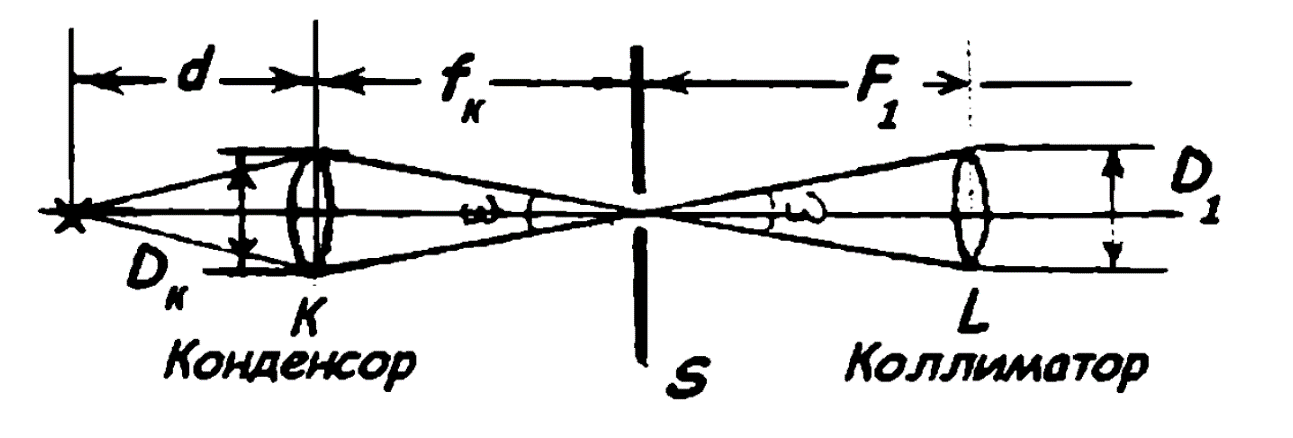
\includegraphics[scale=0.5, trim={0 0 0 5mm}, clip]{2}%
			}
			
		\end{figure}
	
		\newpage

	\section*{Градуировка}
	
		\subsection*{Снятие спектра ртути}
		
		Измеренные в два наблюдения значения углов поворота барабана ($ \alpha $) для линий спектра ртути, соответствующие определенному цвету субъективные оценки интенсивности и табличные длины волн ($ \lambda $):
		
		\begin{center}
	
		\captionof{table}{Снятый спектр ртути} 
		\begin{tabular}{M{2,5 cm}M{3 cm}M{3 cm}M{3,5 cm}M{2,5 cm}} 
			
			\toprule
			
			{\text{Цвет}} & {$ \alpha \text{ (набл. 1), } ^\circ $} & {$ \alpha \text{ (набл. 2), } ^\circ $} & {$ \text{Интенсивность} $} & {$ \lambda, \mathring{A} $} \\
			
			\midrule
			
			Красный & (2932 ± 1) & +8.872 & 16.128 & 1.402 \\
			Красный & (2883 ± 1) & -2.509 & 3.442  & 0.299 \\
			Красный & (2826 ± 1) -0.363 & 1.826  & 0.159 \\
			Красно-оранжевый & (2656 ± 1) & -0.429 & 0.993  & 0.086 \\
			Красно-оранжевый & (2608 ± 1) & 
			Красно-оранжевый & (2584 ± 1)
			Желтая & (2448 ± 1)
			Желтая & (2438 ± 1)
			Зелёный & (2260 ± 1)
			Бирюзовый & (1876 ± 1)
			Бирюзовый & (1838 ± 1)
			Сине-фиолетовый & (1174 ± 1)
			Сине-фиолетовый & (1156 ± 1)
			Сине-фиолетовый & (1142 ± 1)
			Фиолетовый & (741 ± 1)
			Фиолетовый & (680 ± 1)
			Фиолетовый & (619 ± 1)
			
	 		\bottomrule
	 		
		\end{tabular}
		
		\end{center}
	
	
	
\end{document}